% Capitolul 10: Recapitulare Comprehensivă
% Prezentare academică de calitate Harvard
% Program de licență, Academia de Studii Economice din București

\documentclass[9pt, aspectratio=169, t]{beamer}

% Asigură încadrarea conținutului pe diapozitive
\setbeamersize{text margin left=8mm, text margin right=8mm}

%=============================================================================
% CONFIGURARE TEMĂ ȘI STIL
%=============================================================================
\usetheme{default}
% Using default theme for clean header/footer control

% Color Palette (matching Redispatch PDF)
\definecolor{MainBlue}{RGB}{26, 58, 110}
\definecolor{AccentBlue}{RGB}{26, 58, 110}
\definecolor{IDAred}{RGB}{205, 0, 0}
\definecolor{DarkGray}{RGB}{51, 51, 51}
\definecolor{MediumGray}{RGB}{128, 128, 128}
\definecolor{LightGray}{RGB}{248, 248, 248}
\definecolor{VeryLightGray}{RGB}{235, 235, 235}
\definecolor{KeynoteGray}{RGB}{218, 218, 218}
\definecolor{SectionGray}{RGB}{120, 120, 120}
\definecolor{FooterGray}{RGB}{100, 100, 100}
\definecolor{Crimson}{RGB}{220, 53, 69}
\definecolor{Forest}{RGB}{46, 125, 50}
\definecolor{Amber}{RGB}{181, 133, 63}
\definecolor{Orange}{RGB}{230, 126, 34}
\definecolor{Purple}{RGB}{142, 68, 173}

% Gradient background (exact Keynote 315° gradient: white to RGB 218,218,218)
\setbeamertemplate{background}{%
    \begin{tikzpicture}[remember picture, overlay]
        \shade[shading=axis, shading angle=315,
        top color=white, bottom color=KeynoteGray]
        (current page.south west) rectangle (current page.north east);
    \end{tikzpicture}%
}
% Fallback solid color for compatibility
\setbeamercolor{background canvas}{bg=}

\setbeamercolor{palette primary}{bg=MainBlue, fg=white}
\setbeamercolor{palette secondary}{bg=MainBlue!85, fg=white}
\setbeamercolor{palette tertiary}{bg=MainBlue!70, fg=white}
\setbeamercolor{structure}{fg=MainBlue}
\setbeamercolor{title}{fg=IDAred}
\setbeamercolor{frametitle}{fg=IDAred, bg=}
\setbeamercolor{block title}{bg=MainBlue, fg=white}
\setbeamercolor{block body}{bg=VeryLightGray, fg=DarkGray}
\setbeamercolor{block title alerted}{bg=Crimson, fg=white}
\setbeamercolor{block body alerted}{bg=Crimson!8, fg=DarkGray}
\setbeamercolor{block title example}{bg=Forest, fg=white}
\setbeamercolor{block body example}{bg=Forest!8, fg=DarkGray}
\setbeamercolor{item}{fg=MainBlue}

% Footer colors (override Madrid theme blue)
\setbeamercolor{author in head/foot}{fg=FooterGray, bg=}
\setbeamercolor{title in head/foot}{fg=FooterGray, bg=}
\setbeamercolor{date in head/foot}{fg=FooterGray, bg=}
\setbeamercolor{section in head/foot}{fg=FooterGray, bg=}
\setbeamercolor{subsection in head/foot}{fg=FooterGray, bg=}

% Bullet styles (apply everywhere including blocks)
\setbeamertemplate{itemize item}{\color{MainBlue}$\boxdot$}
\setbeamertemplate{itemize subitem}{\color{MainBlue}$\blacktriangleright$}
\setbeamertemplate{itemize subsubitem}{\color{MainBlue}\tiny$\bullet$}
\setbeamertemplate{itemize/enumerate body begin}{\normalsize}
\setbeamertemplate{itemize/enumerate subbody begin}{\normalsize}

% Item spacing - compact style
\setlength{\leftmargini}{10pt}       % Level 1: minimal indent
\setlength{\leftmarginii}{10pt}      % Level 2: minimal additional indent

\setbeamertemplate{navigation symbols}{}

%=============================================================================
% CUSTOM HEADLINE
%=============================================================================
\setbeamertemplate{headline}{%
    \vskip10pt%
    \hbox to \paperwidth{%
        \hskip0.5cm%
        {\small\color{FooterGray}\renewcommand{\hyperlink}[2]{##2}\insertsectionhead}%
        \hfill%
        \textcolor{FooterGray}{\small\insertframenumber}%
        \hskip0.5cm%
    }%
    \vskip4pt%
    {\color{FooterGray}\hrule height 0.4pt}%
}

%=============================================================================
% CUSTOM FOOTER
%=============================================================================
\usepackage{fontawesome5}

\setbeamertemplate{footline}{%
    {\color{FooterGray}\hrule height 0.4pt}%
    \vskip4pt%
    \hbox to \paperwidth{%
        \hskip0.5cm%
        \textcolor{FooterGray}{\small Analiza și Prognoza Seriilor de Timp}%
        \hfill%
        \raisebox{-0.1em}{%
            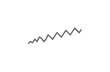
\begin{tikzpicture}[x=0.08em, y=0.08em, line width=0.4pt]
                \draw[FooterGray] (0,3) -- (1,4) -- (2,3.5) -- (3,5) -- (4,4) -- (5,6) -- (6,5.5) -- (7,4) -- (8,5) -- (9,7) -- (10,6) -- (11,5) -- (12,6.5) -- (13,8) -- (14,7) -- (15,6) -- (16,7.5) -- (17,9) -- (18,8) -- (19,7) -- (20,8.5) -- (21,10) -- (22,9) -- (23,8) -- (24,9.5);
            \end{tikzpicture}%
        }%
        \hskip0.5cm%
    }%
    \vskip6pt%
}

%=============================================================================
% PACHETE
%=============================================================================
\usepackage[utf8]{inputenc}
\usepackage[T1]{fontenc}
\usepackage{amsmath, amssymb, amsthm}
\usepackage{mathtools}
\usepackage{bm}
\usepackage{tikz}
\usetikzlibrary{arrows.meta, positioning, shapes, calc, decorations.pathreplacing, shadings}
\usepackage{booktabs}
\usepackage{multirow}
\usepackage{array}
\usepackage{graphicx}
\usepackage{hyperref}
\usepackage{colortbl}
\hypersetup{colorlinks=true, linkcolor=MainBlue, urlcolor=MainBlue}
\graphicspath{{../../logos/}{../../charts/}}
\hfuzz=2pt  % Suppress tiny overfull warnings (<2pt)

%=============================================================================
%=============================================================================
% Usage: \quantlet{QuantletName}{https://github.com/...}
\newcommand{\quantlet}[2]{%
    \hfill\href{#2}{\raisebox{-0.15em}{\includegraphics[height=0.7em]{ql_logo.png}}\textcolor{MainBlue}{\tiny\ #1}}%
}


%=============================================================================
% PAGINĂ TITLU PERSONALIZATĂ
%=============================================================================
\defbeamertemplate*{title page}{hybrid}[1][]
{
    \vspace{0.2cm}
    % Logos row - top header (with clickable links)
    \begin{center}
        \href{https://www.ase.ro}{\includegraphics[height=1.0cm]{ase_logo.png}}\hspace{0.3cm}%
        \href{https://theida.net}{\includegraphics[height=1.0cm]{ida_logo.png}}\hspace{0.3cm}%
        \href{https://blockchain-research-center.com}{\includegraphics[height=1.0cm]{brc_logo.png}}\hspace{0.3cm}%
        \href{https://www.ai4efin.ase.ro}{\includegraphics[height=1.0cm]{ai4efin_logo.png}}\hspace{0.3cm}%
        \href{https://ipe.ro/new}{\includegraphics[height=1.0cm]{acad_logo.png}}\hspace{0.3cm}%
        \href{https://www.digital-finance-msca.com}{\includegraphics[height=1.0cm]{msca_logo.png}}%
    \end{center}

    \vspace{0.6cm}

    % Main title with Q logos on sides (with clickable links)
    \begin{center}
        \begin{minipage}{0.1\textwidth}
            \centering
            \href{https://quantlet.com}{\includegraphics[height=1.1cm]{ql_logo.png}}
        \end{minipage}%
        \begin{minipage}{0.78\textwidth}
            \centering
            {\LARGE\bfseries\usebeamercolor[fg]{title}\inserttitle}

            \vspace{0.3cm}

            {\usebeamerfont{subtitle}\usebeamercolor[fg]{title}\insertsubtitle}
        \end{minipage}%
        \begin{minipage}{0.1\textwidth}
            \centering
            \href{https://quantinar.com}{\includegraphics[height=1.1cm]{qr_logo.png}}
        \end{minipage}
    \end{center}

    \vspace{0.6cm}

    % Authors (left aligned)
    \hspace{0.5cm}{\usebeamerfont{author}\insertauthor}

    \vspace{0.3cm}

    % Institute/Affiliations (left aligned)
    \hspace{0.5cm}\begin{minipage}[t]{0.9\textwidth}
        \raggedright\small\insertinstitute
    \end{minipage}
}

%=============================================================================
% MEDII PENTRU TEOREME
%=============================================================================
\theoremstyle{definition}
\setbeamertemplate{theorems}[numbered]
\newtheorem{defn}{Definiție}
\newtheorem{thm}{Teoremă}
\newtheorem{prop}{Propoziție}
\newtheorem{rmk}{Observație}

%=============================================================================
% COMENZI PERSONALIZATE
%=============================================================================
\newcommand{\E}{\mathbb{E}}
\newcommand{\Var}{\text{Var}}
\newcommand{\Cov}{\text{Cov}}
\newcommand{\Corr}{\text{Corr}}
\newcommand{\R}{\mathbb{R}}
\newcommand{\N}{\mathbb{N}}
\newcommand{\Z}{\mathbb{Z}}
\newcommand{\RMSE}{\text{RMSE}}
\newcommand{\MAE}{\text{MAE}}
\newcommand{\MAPE}{\text{MAPE}}

%=============================================================================
% INFORMAȚII TITLU
%=============================================================================
\title[Analiza Seriilor de Timp]{Analiza și Prognoza Seriilor de Timp}
\subtitle{Capitolul 10: Recapitulare Comprehensivă}
\author[D.T. Pele]{Daniel Traian PELE}
\institute{Academia de Studii Economice din București\\
IDA Institute Digital Assets\\
Blockchain Research Center\\
AI4EFin Artificial Intelligence for Energy Finance\\
Academia Română, Institutul de Prognoză Economică\\
MSCA Digital Finance}
\date{}

\begin{document}

% Title page (no header/footer)
{
\setbeamertemplate{headline}{}
\setbeamertemplate{footline}{}
\begin{frame}
    \titlepage
\end{frame}
}

%=============================================================================
% OUTLINE
%=============================================================================
\begin{frame}{Cuprins}
    \vspace{-0.3cm}
    {\small
    \begin{columns}[T]
        \begin{column}{0.48\textwidth}
            \begin{block}{Fundamente}
                \begin{itemize}\setlength{\itemsep}{3pt}
                    \item Metodologia Prognozei
                    \item Studiu de Caz 1: Volatilitatea Bitcoin (GARCH)
                    \item Studiu de Caz 2: Ciclurile Petelor Solare (Fourier)
                \end{itemize}
            \end{block}
        \end{column}
        \begin{column}{0.48\textwidth}
            \begin{exampleblock}{Aplicații}
                \begin{itemize}\setlength{\itemsep}{3pt}
                    \item Studiu de Caz 3: Șomajul (Prophet)
                    \item Studiu de Caz 4: Analiză Multivariată (VAR)
                    \item Sinteză și Ghid
                    \item Quiz
                \end{itemize}
            \end{exampleblock}
        \end{column}
    \end{columns}
    }
\end{frame}

%=============================================================================
% SECTION 1: METHODOLOGY
%=============================================================================
\section{Metodologia Prognozei}

\begin{frame}{Abordarea științifică a prognozei}
    \begin{block}{Întrebarea de Cercetare}
        \begin{itemize}\setlength{\itemsep}{0pt}
            \item Cum putem \textbf{evalua riguros} performanța prognozei evitând supraajustarea?
        \end{itemize}
    \end{block}

    \vspace{0.3cm}

    \begin{alertblock}{Problema Fundamentală}
        \begin{itemize}
            \item Ajustarea în eșantion $\neq$ Performanța în afara eșantionului
            \item Modelele pot ``memora'' datele de antrenament fără a învăța tipare
            \item \textbf{Soluție}: Metodologia corectă train/validation/test
        \end{itemize}
    \end{alertblock}

    \vspace{0.3cm}

    \begin{exampleblock}{Principiu Cheie}
        \begin{itemize}\setlength{\itemsep}{0pt}
            \item ``Setul de test trebuie să rămână \textbf{neatins} până la evaluarea finală.''
            \item Practică standard în machine learning și econometrie
        \end{itemize}
    \end{exampleblock}
\end{frame}

\begin{frame}{Cadrul Train/Validation/Test}
    \vspace{-0.3cm}
    \begin{center}
        \includegraphics[width=0.72\textwidth]{../charts/train_val_test_split.pdf}
    \end{center}
    \vspace{-0.3cm}
    {\footnotesize
    \begin{columns}[T]
        \column{0.33\textwidth}
        \begin{block}{Set Antrenament}
            \begin{itemize}\setlength{\itemsep}{0pt}
                \item Estimare parametri
                \item Cea mai mare parte
            \end{itemize}
        \end{block}

        \column{0.33\textwidth}
        \begin{block}{Set Validare}
            \begin{itemize}\setlength{\itemsep}{0pt}
                \item Comparare modele
                \item Ajustare hiperparam
            \end{itemize}
        \end{block}

        \column{0.33\textwidth}
        \begin{block}{Set Test}
            \begin{itemize}\setlength{\itemsep}{0pt}
                \item \textbf{Păstrat}
                \item Metrici finale
            \end{itemize}
        \end{block}
    \end{columns}
    }
    \quantlet{TSA\_ch10\_train\_val\_test\_split}{https://github.com/QuantLet/TSA/tree/main/TSA_ch10_train_val_test_split}
\end{frame}

\begin{frame}{Metrici de evaluare}
    \begin{defn}[Metrici ale Erorii de Prognoză]
        \begin{itemize}\setlength{\itemsep}{0pt}
            \item \textbf{Date}: Fie $y_t$ valorile reale, $\hat{y}_t$ prognozele
        \end{itemize}
        \vspace{-0.2cm}
        \begin{align*}
            \RMSE = \sqrt{\frac{1}{n}\sum_{t}(y_t - \hat{y}_t)^2}, \quad
            \MAE = \frac{1}{n}\sum_{t}|y_t - \hat{y}_t|, \quad
            \MAPE = \frac{100\%}{n}\sum_{t}\left|\frac{y_t - \hat{y}_t}{y_t}\right|
        \end{align*}
    \end{defn}

    \begin{columns}[T]
        \column{0.5\textwidth}
        \begin{exampleblock}{Când să folosim}
            \begin{itemize}
                \item \textbf{RMSE}: Penalizează erorile mari
                \item \textbf{MAE}: Robust la outlieri
                \item \textbf{MAPE}: Independent de scală (\%)
            \end{itemize}
        \end{exampleblock}

        \column{0.5\textwidth}
        \begin{alertblock}{Atenție}
            \begin{itemize}
                \item MAPE nedefinit când $y_t = 0$
                \item Comparați pe \textbf{același} set test
                \item Raportați metrici \textbf{out-of-sample}
            \end{itemize}
        \end{alertblock}
    \end{columns}
\end{frame}

%=============================================================================
% SECTION 2: BITCOIN VOLATILITY
%=============================================================================
\section{Studiu de Caz 1: Volatilitatea Bitcoin (GARCH)}

\begin{frame}{Bitcoin: definirea problemei}
    \begin{block}{Întrebarea de Cercetare}
        \begin{itemize}\setlength{\itemsep}{0pt}
            \item Putem prognoza \textbf{volatilitatea} Bitcoin folosind modele GARCH?
        \end{itemize}
    \end{block}

    \vspace{0.2cm}

    \begin{columns}[T]
        \column{0.5\textwidth}
        \textbf{Caracteristicile Datelor}
        \begin{itemize}
            \item Sursă: Yahoo Finance (BTC-USD)
            \item Perioadă: Ian 2019 -- Ian 2025
            \item Frecvență: Zilnică
            \item Observații: $\approx 2.200$ zile
        \end{itemize}

        \vspace{0.3cm}

        \textbf{Fapte stilizate}
        \begin{itemize}
            \item Randamente: medie aproape zero
            \item Cozi groase (curtosis $> 3$)
            \item Clustering al volatilității
        \end{itemize}

        \column{0.5\textwidth}
        \begin{alertblock}{Insight Cheie}
            \begin{itemize}\setlength{\itemsep}{0pt}
                \item \textbf{Randamentele financiare} sunt de obicei:
                \begin{itemize}
                    \item Impredictibile în medie
                    \item Predictibile în varianță
                \end{itemize}
                \item $\succ$ Focus pe \textbf{prognoză volatilității}
            \end{itemize}
        \end{alertblock}
    \end{columns}
\end{frame}

\begin{frame}{Bitcoin: volatility clustering}
    \vspace{-0.3cm}
    \begin{center}
        \includegraphics[width=0.65\textwidth]{../charts/btc_returns.pdf}
    \end{center}
    \vspace{-0.3cm}
    {\footnotesize
    \begin{exampleblock}{Observație}
        \begin{itemize}\setlength{\itemsep}{0pt}
            \item Randamentele mari tind să urmeze randamente mari, cele mici urmează cele mici
            \item Acesta este \textbf{volatility clustering} $\succ$ fenomenul pe care GARCH îl captează
        \end{itemize}
    \end{exampleblock}
    }
    \quantlet{TSA\_ch10\_btc\_returns}{https://github.com/QuantLet/TSA/tree/main/TSA_ch10_btc_returns}
\end{frame}

\begin{frame}{Bitcoin: dovezi pentru GARCH}
    \vspace{-0.3cm}
    {\scriptsize
    \begin{columns}[T]
        \column{0.5\textwidth}
        \begin{center}
            \includegraphics[width=0.75\textwidth]{../charts/btc_squared_returns.pdf}
        \end{center}
        \vspace{-0.4cm}
        \begin{block}{Randamente pătrate}
            \begin{itemize}\setlength{\itemsep}{0pt}
                \item $r_t^2$ sunt proxy pentru volatilitate $\sigma_t^2$
                \item Vârfurile se grupează
            \end{itemize}
        \end{block}

        \column{0.5\textwidth}
        \begin{center}
            \includegraphics[width=0.75\textwidth]{../charts/btc_acf_squared.pdf}
        \end{center}
        \vspace{-0.4cm}
        \begin{block}{ACF}
            \begin{itemize}\setlength{\itemsep}{0pt}
                \item Barele depășesc benzile albastre $\succ$ autocorelație semnificativă
            \end{itemize}
        \end{block}
    \end{columns}

    \vspace{-0.2cm}

    \begin{alertblock}{De ce GARCH?}
        \begin{itemize}\setlength{\itemsep}{0pt}
            \item Dacă $r_t^2$ ar fi zgomot alb, ACF ar fi zero
            \item ACF semnificativ: \textbf{volatilitatea trecută prezice volatilitatea viitoare} $\succ$ GARCH captează asta!
        \end{itemize}
    \end{alertblock}
    }
    \quantlet{TSA\_ch10\_btc\_acf\_squared}{https://github.com/QuantLet/TSA/tree/main/TSA_ch10_btc_acf_squared}
\end{frame}

\begin{frame}{Specificarea modelului GARCH}
    \vspace{-0.1cm}
    \begin{defn}[Modelul GARCH(p,q)]
        \begin{itemize}\setlength{\itemsep}{0pt}
            \item \textbf{Date}: Fie $r_t$ randamentele. Modelul GARCH(p,q) este:
        \end{itemize}
        \vspace{-0.2cm}
        \begin{align*}
            r_t &= \mu + \varepsilon_t, \quad \varepsilon_t = \sigma_t z_t, \quad z_t \sim N(0,1) \\[0.2cm]
            \sigma_t^2 &= \omega + \sum_{i=1}^{q}\alpha_i \varepsilon_{t-i}^2 + \sum_{j=1}^{p}\beta_j \sigma_{t-j}^2
        \end{align*}
        \vspace{-0.3cm}
        \begin{itemize}\setlength{\itemsep}{0pt}
            \item \textbf{Condiții}: $\omega > 0$, $\alpha_i \geq 0$, $\beta_j \geq 0$, și $\sum_{i=1}^{q}\alpha_i + \sum_{j=1}^{p}\beta_j < 1$
        \end{itemize}
    \end{defn}

    \vspace{0.1cm}

    {\small
    \begin{columns}[T]
        \column{0.5\textwidth}
        \begin{block}{Variante de Model}
            \begin{itemize}\setlength{\itemsep}{0pt}
                \item \textbf{GARCH(1,1)}: Cel mai comun
                \item \textbf{GJR-GARCH}: Efect de levier
                \item \textbf{EGARCH}: Șocuri asimetrice
            \end{itemize}
        \end{block}

        \column{0.5\textwidth}
        \begin{exampleblock}{Interpretare}
            \begin{itemize}\setlength{\itemsep}{0pt}
                \item $\alpha$: Impactul șocurilor trecute
                \item $\beta$: Persistența volatilității
                \item $\alpha + \beta \approx 1$: Persistență înaltă
            \end{itemize}
        \end{exampleblock}
    \end{columns}
    }
\end{frame}

\begin{frame}{Bitcoin: împărțirea datelor și staționaritate}
    \begin{columns}[T]
        \column{0.5\textwidth}
        \begin{block}{Împărțirea Datelor}
            \begin{center}
            \begin{tabular}{lrr}
                \toprule
                \textbf{Set} & \textbf{Perioadă} & \textbf{N} \\
                \midrule
                Antrenament (70\%) & 2019-01 -- 2023-03 & 1.543 \\
                Validare (20\%) & 2023-03 -- 2024-06 & 441 \\
                Test (10\%) & 2024-06 -- 2025-01 & 221 \\
                \midrule
                \textbf{Total} & & \textbf{2.205} \\
                \bottomrule
            \end{tabular}
            \end{center}
        \end{block}

        \column{0.5\textwidth}
        \begin{block}{Teste de Staționaritate}
            \begin{center}
            \begin{tabular}{lcc}
                \toprule
                \textbf{Serie} & \textbf{ADF} & \textbf{Rezultat} \\
                \midrule
                Prețuri & $p = 0.50$ & Non-staționară \\
                Randamente & $p < 0.01$ & \textcolor{Forest}{Staționară} \\
                \bottomrule
            \end{tabular}
            \end{center}

            \vspace{0.3cm}

            $\succ$ Modelăm \textbf{randamente}, nu prețuri
        \end{block}
    \end{columns}

    \vspace{0.3cm}

    \begin{alertblock}{De ce Contează Staționaritatea}
        \begin{itemize}\setlength{\itemsep}{0pt}
            \item \textbf{GARCH}: necesită input slab staționar
            \item \textbf{Prețuri vs Randamente}: Prețurile urmează random walk, randamentele sunt staționare
        \end{itemize}
    \end{alertblock}
\end{frame}

\begin{frame}{Bitcoin: selectarea modelului pe setul de validare}
    \begin{block}{Metodologie}
        \begin{itemize}\setlength{\itemsep}{0pt}
            \item Estimăm fiecare model pe \textbf{datele de antrenament}, evaluăm pe \textbf{setul de validare}
        \end{itemize}
    \end{block}

    \vspace{0.3cm}

    \begin{center}
    \begin{tabular}{lcccl}
        \toprule
        \textbf{Model} & \textbf{AIC} & \textbf{BIC} & \textbf{Val MAE} & \textbf{Selectare} \\
        \midrule
        GARCH(1,1) & 6.994,8 & 7.020,6 & \textbf{2,638} & \cellcolor{Forest!20}\textbf{Cel mai bun} \\
        GARCH(2,1) & 6.993,7 & 7.024,6 & 2,640 & \\
        GJR-GARCH(1,1) & 6.983,7 & 7.014,6 & 2,669 & \\
        EGARCH(1,1) & --- & --- & --- & Eșuat$^*$ \\
        \bottomrule
    \end{tabular}
    \end{center}

    \vspace{0.1cm}
    {\footnotesize $^*$Prognoze analitice indisponibile pentru $h > 1$}

    \vspace{0.3cm}

    \begin{exampleblock}{Rezultat}
        \begin{itemize}\setlength{\itemsep}{0pt}
            \item \textbf{GARCH(1,1)} selectat pe baza celui mai mic MAE de validare pentru prognozele de volatilitate
        \end{itemize}
    \end{exampleblock}
\end{frame}

\begin{frame}{Bitcoin: evaluarea finală pe setul de test}
    \vspace{-0.3cm}
    \begin{center}
        \includegraphics[width=0.52\textwidth]{../charts/garch_forecast.pdf}
    \end{center}
    \vspace{-0.3cm}
    {\footnotesize
    \begin{columns}[T]
        \column{0.5\textwidth}
        \begin{block}{Parametri}
            \begin{itemize}\setlength{\itemsep}{0pt}
                \item $\omega=0,87$, $\alpha=0,09$, $\beta=0,84$
                \item $\alpha + \beta = 0,93$ (persistență înaltă)
            \end{itemize}
        \end{block}

        \column{0.5\textwidth}
        \begin{exampleblock}{Performanță Test}
            \begin{itemize}\setlength{\itemsep}{0pt}
                \item MAE = 1,82, RMSE = 2,14
                \item Prognoză urmărește bine volatilitatea realizată
            \end{itemize}
        \end{exampleblock}
    \end{columns}
    }
    \quantlet{TSA\_ch10\_garch\_forecast}{https://github.com/QuantLet/TSA/tree/main/TSA_ch10_garch_forecast}
\end{frame}

\begin{frame}{GARCH: prognozele multi-step converg}
    \vspace{-0.2cm}
    \begin{center}
        \includegraphics[width=0.48\textwidth]{../charts/garch_convergence.pdf}
    \end{center}
    \vspace{-0.3cm}
    {\footnotesize
    \begin{exampleblock}{Insight Cheie}
        \begin{itemize}\setlength{\itemsep}{0pt}
            \item Prognozele multi-step converg la $\bar{\sigma}^2 = \frac{\omega}{1-\alpha-\beta}$
            \item Soluția: prognoze rolling one-step-ahead
        \end{itemize}
    \end{exampleblock}
    }
    \quantlet{TSA\_ch10\_garch\_convergence}{https://github.com/QuantLet/TSA/tree/main/TSA_ch10_garch_convergence}
\end{frame}

\begin{frame}{GARCH: soluția rolling one-step-ahead}
    \begin{center}
        \includegraphics[width=0.85\textwidth]{../charts/rolling_vs_multistep.pdf}
    \end{center}

    \begin{columns}[T]
        \column{0.5\textwidth}
        \begin{exampleblock}{Rolling 1-Step (Stânga)}
            \begin{itemize}\setlength{\itemsep}{0pt}
                \item Re-estimare la fiecare $t$ \textcolor{Forest}{(dinamic)}
            \end{itemize}
        \end{exampleblock}

        \column{0.5\textwidth}
        \begin{block}{Multi-Step (Dreapta)}
            \begin{itemize}\setlength{\itemsep}{0pt}
                \item Converge la $\bar{\sigma}^2$ \textcolor{Crimson}{(plat)}
            \end{itemize}
        \end{block}
    \end{columns}
    \quantlet{TSA\_ch10\_rolling\_vs\_multistep}{https://github.com/QuantLet/TSA/tree/main/TSA_ch10_rolling_vs_multistep}
\end{frame}

\begin{frame}{Bitcoin: Concluzii cheie}
    \begin{columns}[T]
        \column{0.6\textwidth}
        \begin{block}{Sumar}
            \begin{enumerate}
                \item \textbf{Randamentele sunt staționare}; prețurile nu
                \item \textbf{GARCH(1,1)} depășește variantele mai complexe
                \item \textbf{Persistență înaltă} ($\alpha + \beta = 0,93$)
                \item Volatilitatea este \textbf{predictibilă} chiar când randamentele nu sunt
            \end{enumerate}
        \end{block}

        \vspace{0.3cm}

        \begin{exampleblock}{Implicații Practice}
            \begin{itemize}
                \item Managementul riscului: VaR, Expected Shortfall
                \item Evaluarea opțiunilor necesită prognoze de volatilitate
                \item Optimizarea portofoliului cu risc variabil în timp
            \end{itemize}
        \end{exampleblock}

        \column{0.4\textwidth}
        \begin{alertblock}{Limitări}
            \begin{itemize}
                \item GARCH presupune șocuri \textbf{simetrice}
                \item Nu captează \textbf{salturi}
                \item Distribuția normală poate fi restrictivă
            \end{itemize}
        \end{alertblock}

        \vspace{0.3cm}

        \begin{block}{Extensii}
            \begin{itemize}
                \item Inovații Student-t
                \item Volatilitate realizată
                \item Modele HAR
            \end{itemize}
        \end{block}
    \end{columns}
\end{frame}

\begin{frame}{Bitcoin: Fapte stilizate GARCH}
    \vspace{-0.3cm}
    {\scriptsize
    \begin{columns}[T]
        \column{0.5\textwidth}
        \begin{center}
            \includegraphics[width=0.75\textwidth]{../charts/btc_squared_returns.pdf}
        \end{center}
        \vspace{-0.3cm}
        \begin{block}{Observație}
            \begin{itemize}\setlength{\itemsep}{0pt}
                \item $r_t^2$ ca proxy pentru volatilitate
                \item Observați volatility clustering
            \end{itemize}
        \end{block}

        \column{0.5\textwidth}
        \begin{block}{Fapte stilizate Financiare}
            \begin{enumerate}\setlength{\itemsep}{0pt}
                \item \textbf{Clustering volatilitate}: Mișcări mari urmează mișcări mari
                \item \textbf{Cozi groase}: Mai multe extreme decât Normala
                \item \textbf{Efect leverage}: Randamente negative $\succ$ volatilitate mai mare
                \item \textbf{Reversie la medie}: Volatilitatea revine la medie
            \end{enumerate}
        \end{block}
    \end{columns}

    \vspace{-0.2cm}

    \begin{alertblock}{De ce Funcționează GARCH}
        \begin{itemize}\setlength{\itemsep}{0pt}
            \item GARCH captează faptele 1 \& 4
            \item Pentru faptul 3, folosiți GJR-GARCH sau EGARCH
            \item Pentru faptul 2, folosiți inovații Student-t
        \end{itemize}
    \end{alertblock}
    }
\end{frame}

%=============================================================================
% SECTION 3: SUNSPOTS
%=============================================================================
\section{Studiu de Caz 2: Ciclurile Petelor Solare (Fourier)}

\begin{frame}{Pete solare: ciclul solar de 11 ani}
    \vspace{-0.3cm}
    {\scriptsize
    \begin{columns}[T]
        \column{0.55\textwidth}
        \begin{center}
            \includegraphics[width=0.70\textwidth]{../charts/sunspots.pdf}
        \end{center}
        \vspace{-0.3cm}
        \begin{block}{Observație}
            \begin{itemize}\setlength{\itemsep}{0pt}
                \item Liniile punctate marchează vârfurile ciclului ($\approx$11 ani)
            \end{itemize}
        \end{block}

        \column{0.45\textwidth}
        \begin{center}
            \includegraphics[width=0.70\textwidth]{../charts/sunspots_acf.pdf}
        \end{center}
        \vspace{-0.3cm}
        \begin{block}{ACF}
            \begin{itemize}\setlength{\itemsep}{0pt}
                \item Vârfuri la lag 11 și 22, confirmând periodicitatea
            \end{itemize}
        \end{block}
    \end{columns}
    \vspace{-0.3cm}
    \begin{alertblock}{Provocare}
        \begin{itemize}\setlength{\itemsep}{0pt}
            \item \textbf{SARIMA}: $(p,d,q)(P,D,Q)_{11}$ necesită lag-uri sezoniere la 11, 22, 33... $\succ$ prea mulți parametri!
            \item \textbf{Soluție}: Termeni Fourier
        \end{itemize}
    \end{alertblock}
    }
    \quantlet{TSA\_ch10\_sunspots\_acf}{https://github.com/QuantLet/TSA/tree/main/TSA_ch10_sunspots_acf}
\end{frame}

\begin{frame}{Termeni Fourier pentru sezonalitate}
    \vspace{-0.3cm}
    \begin{center}
        \includegraphics[width=0.35\textwidth]{../charts/fourier_terms.pdf}
    \end{center}
    \vspace{-0.4cm}
    {\scriptsize
    \begin{columns}[T]
        \column{0.55\textwidth}
        \begin{block}{Cum funcționează}
            \begin{itemize}\setlength{\itemsep}{0pt}
                \item \textbf{Aproximare}: Orice tipar periodic cu unde sinus și cosinus
                \item \textbf{Formula}: $S_t = \sum_{k=1}^{K}\left[\alpha_k \sin\!\left(\frac{2\pi k t}{s}\right) + \beta_k \cos\!\left(\frac{2\pi k t}{s}\right)\right]$
            \end{itemize}
        \end{block}

        \column{0.45\textwidth}
        \begin{exampleblock}{Insight Cheie}
            \begin{itemize}\setlength{\itemsep}{0pt}
                \item $K=1$: Undă simplă (2 param)
                \item $K=3$: Formă complexă (6 param)
                \item Pete solare: $s=11$, $K=3$
            \end{itemize}
        \end{exampleblock}
    \end{columns}
    }
    \quantlet{TSA\_ch10\_fourier\_terms}{https://github.com/QuantLet/TSA/tree/main/TSA_ch10_fourier_terms}
\end{frame}

\begin{frame}{Pete solare: selectarea modelului}
    \begin{block}{Metodologie}
        \begin{itemize}\setlength{\itemsep}{0pt}
            \item \textbf{Comparație}: $K = 1, 2, 3, 4$ armonici Fourier pe setul de validare
        \end{itemize}
    \end{block}

    \vspace{0.1cm}

    \begin{columns}[T]
        \column{0.5\textwidth}
        \begin{center}
        \textbf{Împărțirea Datelor}
        \begin{tabular}{lrr}
            \toprule
            \textbf{Set} & \textbf{Perioadă} & \textbf{N} \\
            \midrule
            Antrenament (70\%) & 1900--1975 & 76 \\
            Validare (20\%) & 1976--1997 & 22 \\
            Test (10\%) & 1998--2008 & 11 \\
            \midrule
            \textbf{Total} & & \textbf{109} \\
            \bottomrule
        \end{tabular}
        \end{center}

        \column{0.5\textwidth}
        \begin{center}
        \textbf{Comparație Modele}
        \begin{tabular}{cccc}
            \toprule
            \textbf{K} & \textbf{AIC} & \textbf{Val RMSE} & \\
            \midrule
            1 & 665,9 & 87,15 & \\
            2 & 668,0 & 86,92 & \\
            \rowcolor{Forest!20} 3 & 671,8 & \textbf{86,81} & Cel mai bun \\
            4 & 674,5 & 87,93 & \\
            \bottomrule
        \end{tabular}
        \end{center}
    \end{columns}

    \vspace{0.1cm}

    \begin{exampleblock}{Rezultat}
        \begin{itemize}\setlength{\itemsep}{0pt}
            \item \textbf{K = 3} armonici Fourier selectate (6 parametri pentru ciclul de 11 ani)
        \end{itemize}
    \end{exampleblock}
\end{frame}

\begin{frame}{Pete solare: rezultate prognoză}
    \vspace{-0.3cm}
    \begin{center}
        \includegraphics[width=0.52\textwidth]{../charts/sunspot_forecast.pdf}
    \end{center}
    \vspace{-0.3cm}
    {\footnotesize
    \begin{columns}[T]
        \column{0.5\textwidth}
        \begin{block}{Model}
            \begin{itemize}\setlength{\itemsep}{0pt}
                \item \textbf{ARIMA(2,0,1)} + 3 termeni Fourier
                \begin{itemize}
                    \item Captează dinamica ciclului de 11 ani
                \end{itemize}
            \end{itemize}
        \end{block}

        \column{0.5\textwidth}
        \begin{exampleblock}{Performanță Test}
            \begin{itemize}\setlength{\itemsep}{0pt}
                \item \textbf{RMSE} = 31,10, \textbf{MAE} = 25,83
                \begin{itemize}
                    \item Modelul urmărește tiparul general al ciclului
                \end{itemize}
            \end{itemize}
        \end{exampleblock}
    \end{columns}
    }
    \quantlet{TSA\_ch10\_sunspot\_forecast}{https://github.com/QuantLet/TSA/tree/main/TSA_ch10_sunspot_forecast}
\end{frame}

\begin{frame}{Pete solare: concluzii cheie}
    \begin{columns}[T]
        \column{0.5\textwidth}
        \begin{block}{Când să Folosiți Termeni Fourier}
            \begin{itemize}
                \item Perioada sezonieră $s$ este \textbf{lungă} (ex: 11 ani, 52 săptămâni)
                \item SARIMA ar necesita prea multe lag-uri sezoniere
                \item Tiparul este \textbf{neted și periodic}
                \item Trebuie capturate cicluri multiple
            \end{itemize}
        \end{block}

        \vspace{0.2cm}

        \begin{alertblock}{Alegerea lui K}
            \begin{itemize}\setlength{\itemsep}{0pt}
                \item \textbf{Strategie}: Începeți cu $K=1$, creșteți progresiv
                \begin{itemize}
                    \item Opriți când eroarea de validare nu mai scade
                    \item $K$ prea mare = supraajustare
                \end{itemize}
            \end{itemize}
        \end{alertblock}

        \column{0.5\textwidth}
        \begin{exampleblock}{Fourier vs SARIMA}
            \begin{center}
            \begin{tabular}{lcc}
                \toprule
                & \textbf{Fourier} & \textbf{SARIMA} \\
                \midrule
                Sezoane lungi & \checkmark & $\times$ \\
                Sezoane scurte & OK & \checkmark \\
                Parametri & $2K$ & Mulți \\
                Flexibilitate & Fixă & Adaptivă \\
                \bottomrule
            \end{tabular}
            \end{center}
        \end{exampleblock}

        \vspace{0.2cm}

        \begin{block}{Aplicații}
            \begin{itemize}\setlength{\itemsep}{0pt}
                \item \textbf{Domenii}: Cicluri climatice, cicluri de afaceri, fenomene astronomice
            \end{itemize}
        \end{block}
    \end{columns}
\end{frame}

%=============================================================================
% SECTION 4: UNEMPLOYMENT
%=============================================================================
\section{Studiu de Caz 3: Șomajul (Prophet)}

\begin{frame}{Șomajul: Train / Validation / Test Split}
    \begin{center}
        \includegraphics[width=0.62\textwidth]{../charts/unemployment_train_val_test.pdf}
    \end{center}
    \vspace{-0.4cm}
    {\footnotesize
    \begin{block}{Metodologie}
        \begin{itemize}\setlength{\itemsep}{0pt}
            \item \textbf{Training} (70\%): Estimare modele
            \item \textbf{Validare} (20\%): Selecție model
            \item \textbf{Test} (10\%): Evaluare finală
        \end{itemize}
    \end{block}
    }
    \quantlet{TSA\_ch10\_unemployment\_train\_val\_test}{https://github.com/QuantLet/TSA/tree/main/TSA_ch10_unemployment_train_val_test}
\end{frame}

\begin{frame}{Șomajul: analiză preliminară}
    \begin{center}
        \includegraphics[width=0.65\textwidth]{../charts/unemployment_acf_pacf.pdf}
    \end{center}
    \vspace{-0.3cm}
    {\footnotesize
    \begin{columns}[T]
        \column{0.5\textwidth}
        \begin{block}{Interpretare ACF}
            \begin{itemize}\setlength{\itemsep}{0pt}
                \item Descreștere lentă $\succ$ serie nestaționară. Necesită diferențiere ($d \geq 1$)
            \end{itemize}
        \end{block}

        \column{0.5\textwidth}
        \begin{exampleblock}{Interpretare PACF}
            \begin{itemize}\setlength{\itemsep}{0pt}
                \item Vârf semnificativ la lag 1 sugerează componentă AR(1)
                \item Pattern sezonier la lag 12
            \end{itemize}
        \end{exampleblock}
    \end{columns}
    }
    \quantlet{TSA\_ch10\_unemployment\_acf\_pacf}{https://github.com/QuantLet/TSA/tree/main/TSA_ch10_unemployment_acf_pacf}
\end{frame}

\begin{frame}{Șomajul: teste de staționaritate}
    \vspace{-0.2cm}
    \begin{center}
        \includegraphics[width=0.60\textwidth]{../charts/unemployment_stationarity.pdf}
    \end{center}
    \vspace{-0.2cm}
    \begin{columns}[T]
        \column{0.5\textwidth}
        \begin{alertblock}{Original: ADF p = 0,056}
            \begin{itemize}\setlength{\itemsep}{0pt}
                \item Nestaționară (ACF descreștere lentă)
            \end{itemize}
        \end{alertblock}

        \column{0.5\textwidth}
        \begin{exampleblock}{Diferențiată: ADF p $<$ 0,001}
            \begin{itemize}\setlength{\itemsep}{0pt}
                \item Staționară $\succ$ folosim $d=1$
            \end{itemize}
        \end{exampleblock}
    \end{columns}
    \quantlet{TSA\_ch10\_unemployment\_stationarity}{https://github.com/QuantLet/TSA/tree/main/TSA_ch10_unemployment_stationarity}
\end{frame}

\begin{frame}{Șomajul: selecția modelului (set validare)}
    \begin{center}
        \includegraphics[width=0.58\textwidth]{../charts/sarima_model_selection.pdf}
    \end{center}
    \vspace{-0.4cm}
    {\footnotesize
    \begin{block}{Best: SARIMA(1,1,1)(1,0,0)$_{12}$}
        \begin{itemize}\setlength{\itemsep}{0pt}
            \item Fit pe training (70\%), evaluare pe validare (20\%)
            \item Cel mai bun model selectat după Val RMSE minim
        \end{itemize}
    \end{block}
    }
    \quantlet{TSA\_ch10\_sarima\_model\_selection}{https://github.com/QuantLet/TSA/tree/main/TSA_ch10_sarima_model_selection}
\end{frame}

\begin{frame}{Șomajul: parametrii SARIMA}
    \begin{center}
        \includegraphics[width=0.65\textwidth]{../charts/sarima_parameters.pdf}
    \end{center}

    \begin{block}{SARIMA(1,1,1)(1,0,0)$_{12}$ estimat pe Train+Val (2010-2019)}
        \begin{itemize}\setlength{\itemsep}{0pt}
            \item AR(1): $\phi_1 = -0,86$, MA(1): $\theta_1 = 0,78$, SAR(12): $\Phi_1 = -0,08$ (n.s.)
        \end{itemize}
    \end{block}
    \quantlet{TSA\_ch10\_sarima\_parameters}{https://github.com/QuantLet/TSA/tree/main/TSA_ch10_sarima_parameters}
\end{frame}

\begin{frame}{Șomajul: Diagnosticare SARIMA}
    \begin{center}
        \includegraphics[width=0.40\textwidth]{../charts/sarima_diagnostics.pdf}
    \end{center}
    \vspace{-0.35cm}
    \begin{columns}[T]
        \column{0.5\textwidth}
        \begin{block}{Reziduuri}
            \begin{itemize}\setlength{\itemsep}{0pt}
                \item \textbf{ACF}: Fără autocorelație reziduală
                \item \textbf{Ljung-Box}: $p = 0{,}66$ $\succ$ model bine specificat
            \end{itemize}
        \end{block}

        \column{0.5\textwidth}
        \begin{alertblock}{Q-Q Plot: Non-normalitate}
            \begin{itemize}\setlength{\itemsep}{0pt}
                \item Deviație la cozi datorită \textbf{șocului COVID} (2020)
                \item Reziduurile au distribuție leptokurtotică
            \end{itemize}
        \end{alertblock}
    \end{columns}
    \quantlet{TSA\_ch10\_sarima\_diagnostics}{https://github.com/QuantLet/TSA/tree/main/TSA_ch10_sarima_diagnostics}
\end{frame}

\begin{frame}{Șomajul: prognoza rolling SARIMA}
    \vspace{-0.1cm}
    \begin{center}
        \includegraphics[width=0.68\textwidth]{../charts/sarima_forecast.pdf}
    \end{center}
    \vspace{-0.4cm}
    {\footnotesize
    \begin{alertblock}{Problemă: Ruptura Structurală}
        \begin{itemize}\setlength{\itemsep}{0pt}
            \item Prognoză rolling one-step-ahead (re-estimare la fiecare $t$): \textbf{Test RMSE = 0,12}
        \end{itemize}
    \end{alertblock}
    }
    \quantlet{TSA\_ch10\_sarima\_forecast}{https://github.com/QuantLet/TSA/tree/main/TSA_ch10_sarima_forecast}
\end{frame}

\begin{frame}{Modelul Prophet}
    \begin{defn}[Descompunerea Prophet]
        \begin{itemize}\setlength{\itemsep}{0pt}
            \item \textbf{Model}: $y_t = g(t) + s(t) + h(t) + \varepsilon_t$, \quad $\varepsilon_t \sim N(0, \sigma^2)$
            \item \textbf{Componente}: $g(t)$ = trend, $s(t)$ = sezonalitate, $h(t)$ = sărbători
        \end{itemize}
    \end{defn}

    \vspace{0.2cm}

    \begin{columns}[T]
        \column{0.5\textwidth}
        \begin{block}{Detectare Puncte de Schimbare}
            \begin{itemize}
                \item Selectare automată a locațiilor
                \item \texttt{changepoint\_prior\_scale} controlează flexibilitatea
            \end{itemize}
        \end{block}

        \column{0.5\textwidth}
        \begin{exampleblock}{Avantaje}
            \begin{itemize}
                \item Gestionează date lipsă
                \item Componente interpretabile
                \item Robust la outlieri
            \end{itemize}
        \end{exampleblock}
    \end{columns}
\end{frame}

\begin{frame}{Șomajul: Ajustarea modelului}
    \vspace{-0.1cm}
    {\footnotesize
    \begin{block}{Ajustarea Hiperparametrilor}
        \begin{itemize}\setlength{\itemsep}{0pt}
            \item Ajustăm \texttt{changepoint\_prior\_scale} pe setul de validare
        \end{itemize}
    \end{block}
    }

    \vspace{0.05cm}

    {\footnotesize
    \begin{columns}[T]
        \column{0.5\textwidth}
        \begin{center}
        \textbf{Împărțirea Datelor}
        \begin{tabular}{lrr}
            \toprule
            \textbf{Set} & \textbf{Perioadă} & \textbf{N} \\
            \midrule
            Antrenament (70\%) & 2010-01 -- 2020-06 & 126 \\
            Validare (20\%) & 2020-07 -- 2023-06 & 36 \\
            Test (10\%) & 2023-07 -- 2025-01 & 19 \\
            \midrule
            \textbf{Total} & & \textbf{181} \\
            \bottomrule
        \end{tabular}
        \end{center}

        \column{0.5\textwidth}
        \begin{center}
        \textbf{Comparație Scale}
        \begin{tabular}{ccc}
            \toprule
            \textbf{Scale} & \textbf{Val RMSE} & \\
            \midrule
            0,01 & 4,21 & \\
            0,05 & 3,89 & \\
            \rowcolor{Forest!20} 0,10 & \textbf{3,52} & Cel mai bun \\
            0,30 & 3,67 & \\
            0,50 & 3,81 & \\
            \bottomrule
        \end{tabular}
        \end{center}
    \end{columns}

    \vspace{0.05cm}

    \begin{alertblock}{Interpretare}
        \begin{itemize}\setlength{\itemsep}{0pt}
            \item Scale = 0,10 echilibrează flexibilitatea (captarea șocului COVID) cu stabilitatea
        \end{itemize}
    \end{alertblock}
    }
\end{frame}

\begin{frame}{Șomajul: rezultate prognoză Prophet}
    \vspace{-0.3cm}
    \begin{center}
        \includegraphics[width=0.52\textwidth]{../charts/unemployment_forecast.pdf}
    \end{center}
    \vspace{-0.4cm}
    \begin{block}{Concluzie Cheie}
        \begin{itemize}\setlength{\itemsep}{0pt}
            \item \textbf{Prophet}: se adaptează prin detectare changepoint
            \item \textbf{Test RMSE} = 0,58
        \end{itemize}
    \end{block}
    \quantlet{TSA\_ch10\_unemployment\_forecast}{https://github.com/QuantLet/TSA/tree/main/TSA_ch10_unemployment_forecast}
\end{frame}

\begin{frame}{Șomaj: comparație SARIMA vs Prophet}
    \vspace{-0.3cm}
    \begin{center}
        \includegraphics[width=0.78\textwidth]{../charts/prophet_vs_sarima_unemployment.pdf}
    \end{center}
    \vspace{-0.4cm}
    {\footnotesize
    \begin{columns}[T]
        \column{0.5\textwidth}
        \begin{exampleblock}{SARIMA: RMSE = 0,12}
            \begin{itemize}\setlength{\itemsep}{0pt}
                \item Prognoză rolling performează bine
            \end{itemize}
        \end{exampleblock}

        \column{0.5\textwidth}
        \begin{block}{Prophet: RMSE = 0,12}
            \begin{itemize}\setlength{\itemsep}{0pt}
                \item Se adaptează prin changepoints
            \end{itemize}
        \end{block}
    \end{columns}
    }
    \quantlet{TSA\_ch10\_prophet\_vs\_sarima\_unemployment}{https://github.com/QuantLet/TSA/tree/main/TSA_ch10_prophet_vs_sarima_unemployment}
\end{frame}

\begin{frame}{Prophet: când să-l folosești}
    \begin{columns}[T]
        \column{0.5\textwidth}
        \begin{block}{Cazuri de Utilizare Ideale}
            \begin{itemize}
                \item Date de business cu \textbf{sărbători}
                \item \textbf{Valori lipsă} prezente
                \item Nevoie de componente \textbf{interpretabile}
                \item Prognoze cu \textbf{benzi de incertitudine}
            \end{itemize}
        \end{block}

        \vspace{0.2cm}

        \begin{alertblock}{Atenție: Rupturi Structurale}
            \begin{itemize}\setlength{\itemsep}{0pt}
                \item Prophet gestionează rupturile prin changepoints, dar \textbf{SARIMA l-a depășit} la șomaj (0,12 vs 0,58)
                \item Validați întotdeauna!
            \end{itemize}
        \end{alertblock}

        \column{0.5\textwidth}
        \begin{exampleblock}{Prophet vs ARIMA}
            \begin{center}
            \begin{tabular}{lcc}
                \toprule
                & \textbf{Prophet} & \textbf{ARIMA} \\
                \midrule
                Changepoints & \checkmark & $\times$ \\
                Date lipsă & \checkmark & $\times$ \\
                Sărbători & \checkmark & $\times$ \\
                Viteză & Rapidă & Moderată \\
                Interpretabil & \checkmark & $\times$ \\
                \bottomrule
            \end{tabular}
            \end{center}
        \end{exampleblock}

        \vspace{0.2cm}

        \begin{block}{Parametri cheie}
            \begin{itemize}\setlength{\itemsep}{0pt}
                \item \texttt{changepoint\_prior\_scale}: flexibilitate
                \item \texttt{seasonality\_prior\_scale}: netezime
            \end{itemize}
        \end{block}
    \end{columns}
\end{frame}

%=============================================================================
% SECTION 5: VAR
%=============================================================================
\section{Studiu de Caz 4: Analiză Multivariată (VAR)}

\begin{frame}{VAR: date economice multivariate}
    \begin{center}
        \includegraphics[width=0.42\textwidth]{../charts/economic_vars.pdf}
    \end{center}
    \vspace{-0.3cm}
    \begin{columns}[T]
        \column{0.5\textwidth}
        \begin{block}{Relații Economice}
            \begin{itemize}\setlength{\itemsep}{0pt}
                \item \textbf{Legea Okun}: PIB $\leftrightarrow$ Șomaj
                \item \textbf{Curba Phillips}: Șomaj $\leftrightarrow$ Inflație
            \end{itemize}
        \end{block}

        \column{0.5\textwidth}
        \begin{exampleblock}{De ce VAR?}
            \begin{itemize}\setlength{\itemsep}{0pt}
                \item Fiecare variabilă e atât cauză cât și efect
                \item VAR captează aceste bucle de feedback
            \end{itemize}
        \end{exampleblock}
    \end{columns}
    \quantlet{TSA\_ch10\_economic\_vars}{https://github.com/QuantLet/TSA/tree/main/TSA_ch10_economic_vars}
\end{frame}

\begin{frame}{Specificarea modelului VAR}
    \begin{defn}[Autoregresie Vectorială VAR(p)]
        \begin{itemize}\setlength{\itemsep}{0pt}
            \item \textbf{Date}: Pentru $K$ variabile $\mathbf{y}_t = (y_{1t}, \ldots, y_{Kt})'$:
        \end{itemize}
        \vspace{-0.2cm}
        \begin{equation*}
            \mathbf{y}_t = \mathbf{c} + \mathbf{A}_1\mathbf{y}_{t-1} + \mathbf{A}_2\mathbf{y}_{t-2} + \cdots + \mathbf{A}_p\mathbf{y}_{t-p} + \mathbf{u}_t
        \end{equation*}
        \vspace{-0.3cm}
        \begin{itemize}\setlength{\itemsep}{0pt}
            \item \textbf{Notație}: $\mathbf{A}_i$ sunt matrici de coeficienți $K \times K$, $\mathbf{u}_t \sim N(\mathbf{0}, \boldsymbol{\Sigma})$
        \end{itemize}
    \end{defn}

    \vspace{0.1cm}

    \begin{columns}[T]
        \column{0.5\textwidth}
        \begin{block}{Pentru Sistemul Nostru cu 4 Variabile}
            \begin{itemize}
                \item \textbf{VAR(2)}: 4 constante
                \item $2 \times 4 \times 4 = 32$ coeficienți AR
                \item \textbf{36 parametri total}
            \end{itemize}
        \end{block}

        \column{0.5\textwidth}
        \begin{exampleblock}{Selectarea Lag-ului}
            \begin{itemize}\setlength{\itemsep}{0pt}
                \item Folosim criterii informaționale:
                \begin{itemize}
                    \item AIC: Tinde să supraajusteze
                    \item \textbf{BIC}: Mai simplu
                    \item Cross-validare pe date păstrate
                \end{itemize}
            \end{itemize}
        \end{exampleblock}
    \end{columns}
\end{frame}

\begin{frame}{VAR: selectarea lag-ului și estimare}
    \begin{columns}[T]
        \column{0.5\textwidth}
        \begin{block}{Criterii informaționale}
            \begin{center}
            \begin{tabular}{ccc}
                \toprule
                \textbf{Lag} & \textbf{BIC} & \\
                \midrule
                1 & -4,810 & \\
                \rowcolor{Forest!20} 2 & \textbf{-5,178} & Cel mai bun \\
                3 & -4,633 & \\
                4 & -4,614 & \\
                \bottomrule
            \end{tabular}
            \end{center}
        \end{block}

        \vspace{0.2cm}

        \begin{exampleblock}{Verificare Validare}
            \begin{itemize}\setlength{\itemsep}{0pt}
                \item VAR(2) obține și cel mai mic RMSE de validare
            \end{itemize}
        \end{exampleblock}

        \column{0.5\textwidth}
        \begin{block}{Împărțirea Datelor}
            \begin{center}
            \begin{tabular}{lrr}
                \toprule
                \textbf{Set} & \textbf{Perioadă} & \textbf{N} \\
                \midrule
                Antrenament (70\%) & 2001-T1 -- 2017-T4 & 67 \\
                Validare (20\%) & 2018-T1 -- 2022-T4 & 20 \\
                Test (10\%) & 2023-T1 -- 2025-T1 & 10 \\
                \midrule
                \textbf{Total} & & \textbf{97} \\
                \bottomrule
            \end{tabular}
            \end{center}
        \end{block}
    \end{columns}
\end{frame}

\begin{frame}{Analiza cauzalității Granger}
    \vspace{-0.2cm}
    {\footnotesize
    \begin{columns}[T]
        \column{0.42\textwidth}
        \begin{center}
            \includegraphics[width=0.90\textwidth]{../charts/granger_heatmap.pdf}
        \end{center}
        \vspace{-0.2cm}
        \begin{block}{Interpretare}
            \begin{itemize}\setlength{\itemsep}{0pt}
                \item \textbf{Celule verzi}: $p < 0.10$ (semnificativ)
                \item \textbf{Citire}: rândul cauzează coloana
            \end{itemize}
        \end{block}

        \column{0.58\textwidth}
        \begin{block}{Ce este Cauzalitatea Granger?}
            \begin{itemize}\setlength{\itemsep}{0pt}
                \item $X$ \textbf{cauzează Granger} $Y$ dacă $X$ trecut îmbunătățește predicția lui $Y$ dincolo de $Y$ trecut singur
                \item \textit{Atenție: ``Cauzalitate Granger'' $\neq$ cauzalitate reală!}
            \end{itemize}
        \end{block}

        \vspace{0.05cm}

        \begin{exampleblock}{Concluzii Economice}
            \begin{itemize}\setlength{\itemsep}{0pt}
                \item Șomaj $\succ$ PIB ($p=0,045$): Legea Okun
                \item Fed $\succ$ Inflație ($p=0,087$): Politica monetară funcționează
            \end{itemize}
        \end{exampleblock}
    \end{columns}
    }
    \quantlet{TSA\_ch10\_granger\_heatmap}{https://github.com/QuantLet/TSA/tree/main/TSA_ch10_granger_heatmap}
\end{frame}

\begin{frame}{Funcții de răspuns la impuls (IRF)}
    \vspace{-0.2cm}
    \begin{columns}[T]
        \column{0.6\textwidth}
        \begin{center}
            \includegraphics[width=0.95\textwidth]{../charts/irf_gdp_shock.pdf}
        \end{center}

        \column{0.4\textwidth}
        \begin{block}{Ce este IRF?}
            \begin{itemize}\setlength{\itemsep}{0pt}
                \item Arată cum un șoc de 1 unitate la o variabilă afectează celelalte în timp
            \end{itemize}
        \end{block}

        \vspace{0.1cm}

        \begin{exampleblock}{Efectele Șocului PIB}
            \begin{itemize}\setlength{\itemsep}{0pt}
                \item \textbf{Șomaj} $\downarrow$: Legea Okun
                \item \textbf{Inflație} $\uparrow$: Cerere-pull
                \item \textbf{Rata Fed} $\uparrow$: Regula Taylor
            \end{itemize}
        \end{exampleblock}
    \end{columns}
    \quantlet{TSA\_ch10\_irf\_gdp\_shock}{https://github.com/QuantLet/TSA/tree/main/TSA_ch10_irf_gdp_shock}
\end{frame}

\begin{frame}{IRF: șoc șomaj}
    \vspace{-0.2cm}
    \begin{center}
        \includegraphics[width=0.52\textwidth]{../charts/irf_unemp_shock.pdf}
    \end{center}
    \vspace{-0.5cm}
    \begin{block}{Efecte}
        \begin{itemize}\setlength{\itemsep}{0pt}
            \item $\uparrow$ Șomaj $\succ$ $\downarrow$ PIB (Okun), $\downarrow$ Inflație (Phillips), Fed reduce rata
        \end{itemize}
    \end{block}
    \quantlet{TSA\_ch10\_irf\_unemp\_shock}{https://github.com/QuantLet/TSA/tree/main/TSA_ch10_irf_unemp_shock}
\end{frame}

\begin{frame}{IRF: șoc rată Fed}
    \vspace{-0.2cm}
    \begin{center}
        \includegraphics[width=0.52\textwidth]{../charts/irf_fed_shock.pdf}
    \end{center}
    \vspace{-0.5cm}
    \begin{block}{Politică Monetară}
        \begin{itemize}\setlength{\itemsep}{0pt}
            \item Creștere rată $\succ$ PIB $\downarrow$, Șomaj $\uparrow$, Inflație $\downarrow$
        \end{itemize}
    \end{block}
    \quantlet{TSA\_ch10\_irf\_fed\_shock}{https://github.com/QuantLet/TSA/tree/main/TSA_ch10_irf_fed_shock}
\end{frame}

\begin{frame}{VAR: Prognoza (Train/Val/Test)}
    \vspace{-0.3cm}
    \begin{center}
        \includegraphics[width=0.48\textwidth]{../charts/var_forecast.pdf}
    \end{center}
    \vspace{-0.4cm}
    {\small
    \begin{block}{Prognoză Rolling One-Step-Ahead}
        \begin{itemize}\setlength{\itemsep}{0pt}
            \item VAR captează dinamică PIB-Șomaj
            \item Șocul COVID vizibil în perioadă validare (2020)
        \end{itemize}
    \end{block}
    }
    \quantlet{TSA\_ch10\_var\_forecast}{https://github.com/QuantLet/TSA/tree/main/TSA_ch10_var_forecast}
\end{frame}

\begin{frame}{VAR: rezultate set test}
    \vspace{-0.1cm}
    {\footnotesize
    \begin{block}{Performanță Set Test pe Variabile}
        \begin{center}
        \begin{tabular}{lccc}
            \toprule
            \textbf{Variabilă} & \textbf{RMSE} & \textbf{MAE} & \textbf{Acur. Direcție} \\
            \midrule
            Creștere PIB & 1,33 & 0,99 & 50\% \\
            Șomaj & 0,64 & 0,52 & 50\% \\
            Inflație & 1,56 & 1,12 & 60\% \\
            Rata Fed & 2,59 & 2,45 & 80\% \\
            \midrule
            \textbf{Medie} & \textbf{1,53} & \textbf{1,27} & \textbf{60\%} \\
            \bottomrule
        \end{tabular}
        \end{center}
    \end{block}

    \vspace{0.05cm}

    \begin{columns}[T]
        \column{0.5\textwidth}
        \begin{exampleblock}{Puncte Forte}
            \begin{itemize}\setlength{\itemsep}{0pt}
                \item Captează dinamică între variabile
                \item Acuratețe direcțională bună
                \item Relații interpretabile
            \end{itemize}
        \end{exampleblock}

        \column{0.5\textwidth}
        \begin{alertblock}{Limitări}
            \begin{itemize}\setlength{\itemsep}{0pt}
                \item Mulți parametri (blestemul dimensionalității)
                \item Sensibil la selectarea lag-ului
                \item Perioada COVID dificilă
            \end{itemize}
        \end{alertblock}
    \end{columns}
    }
\end{frame}

%=============================================================================
% SECTION 6: SYNTHESIS
%=============================================================================
\section{Sinteză și Ghid}

\begin{frame}{Cadrul de selectare a modelului}
    \vspace{-0.3cm}
    \begin{center}
    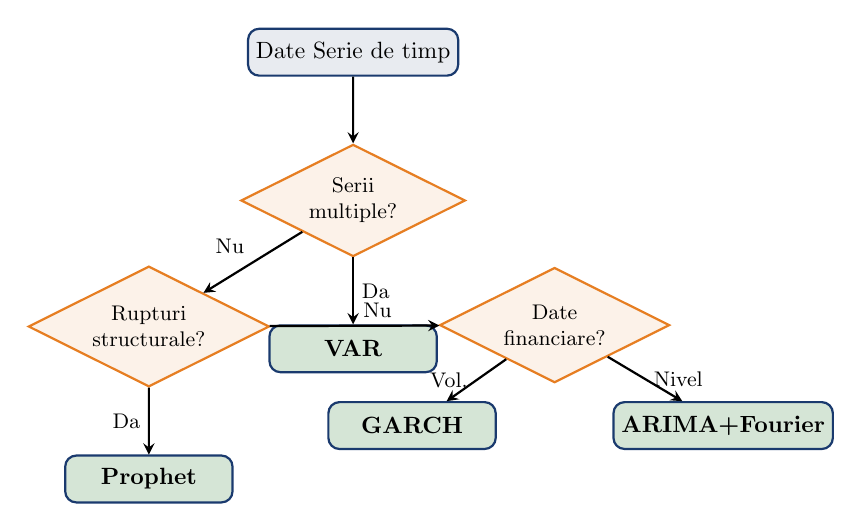
\begin{tikzpicture}[scale=0.85, transform shape,
        node distance=1.0cm,
        box/.style={rectangle, draw=MainBlue, thick, fill=MainBlue!10, rounded corners, minimum width=2.5cm, minimum height=0.7cm, align=center},
        decision/.style={diamond, draw=Orange, thick, fill=Orange!10, aspect=2, align=center, font=\small},
        arrow/.style={->, thick, >=stealth}
    ]
        \node[box] (start) {Date Serie de timp};
        \node[decision, below=of start] (q1) {Serii\\multiple?};
        \node[decision, below left=1.0cm and 1.3cm of q1] (q2) {Rupturi\\structurale?};
        \node[decision, below right=1.0cm and 1.3cm of q1] (q3) {Date\\financiare?};
        \node[box, fill=Forest!20, below=of q1] (var) {\textbf{VAR}};
        \node[box, fill=Forest!20, below=of q2] (prophet) {\textbf{Prophet}};
        \node[box, fill=Forest!20, below left=0.7cm and 0cm of q3] (garch) {\textbf{GARCH}};
        \node[box, fill=Forest!20, below right=0.7cm and 0cm of q3] (arima) {\textbf{ARIMA+Fourier}};
        \draw[arrow] (start) -- (q1);
        \draw[arrow] (q1) -- node[right] {\small Da} (var);
        \draw[arrow] (q1) -- node[above left] {\small Nu} (q2);
        \draw[arrow] (q2) -- node[left] {\small Da} (prophet);
        \draw[arrow] (q2) -- node[above right] {\small Nu} (q3);
        \draw[arrow] (q3) -- node[left] {\small Vol.} (garch);
        \draw[arrow] (q3) -- node[right] {\small Nivel} (arima);
    \end{tikzpicture}
    \end{center}
\end{frame}

\begin{frame}{Sumar: comparație modele}
    \vspace{-0.2cm}
    \begin{columns}[T]
        \column{0.55\textwidth}
        \begin{center}
        \footnotesize
        \begin{tabular}{llll}
            \toprule
            \textbf{Caz} & \textbf{Provocare} & \textbf{Model} & \textbf{RMSE} \\
            \midrule
            Bitcoin & Volatilitate & GARCH & 2,15 \\
            Pete solare & Sezonalitate & Fourier & 31,10 \\
            Șomaj & Ruptură & SARIMA & 0,12 \\
            Economic & Multi-var & VAR & 1,53 \\
            \bottomrule
        \end{tabular}
        \end{center}

        \column{0.45\textwidth}
        \begin{center}
            \includegraphics[width=0.90\textwidth]{../charts/model_comparison.pdf}
        \end{center}
    \end{columns}

    \vspace{0.1cm}

    \begin{exampleblock}{Principiu Cheie}
        \begin{itemize}\setlength{\itemsep}{0pt}
            \item \textbf{Potriviți modelul cu caracteristicile datelor}
            \item Alegeți în funcție de natura problemei și proprietățile datelor
        \end{itemize}
    \end{exampleblock}
    \quantlet{TSA\_ch10\_model\_comparison}{https://github.com/QuantLet/TSA/tree/main/TSA_ch10_model_comparison}
\end{frame}

\begin{frame}{Sinteză: Comparația Modelelor}
    \begin{center}
    \footnotesize
    \begin{tabular}{lcccc}
        \toprule
        \textbf{Caracteristică} & \textbf{GARCH} & \textbf{Fourier} & \textbf{Prophet} & \textbf{VAR} \\
        \midrule
        \textbf{Țintă} & Volatilitate & Nivel & Nivel & Multiple \\
        \textbf{Sezonalitate} & Nu & Da (lungă) & Da (multiplă) & Nu \\
        \textbf{Rupturi structurale} & Nu & Nu & Da & Nu \\
        \textbf{Serii multiple} & Nu & Nu & Nu & Da \\
        \textbf{Interpretabil} & Mediu & Ridicat & Ridicat & Ridicat \\
        \textbf{Parametri} & Puțini & $2K$ & Auto & Mulți \\
        \textbf{Date lipsă} & Nu & Nu & Da & Nu \\
        \midrule
        \textbf{Ideal pentru} & Finanțe & Cicluri & Business & Macro \\
        \bottomrule
    \end{tabular}
    \end{center}

    \vspace{0.3cm}

    \begin{columns}[T]
        \column{0.5\textwidth}
        \begin{block}{Rezultatele Noastre}
            \begin{itemize}
                \item GARCH: MAE=1,82 (volatilitate)
                \item Fourier: RMSE=31,10 (cicluri)
                \item SARIMA: RMSE=0,12 (rupturi)
                \item VAR: RMSE mediu=1,53 (multi)
            \end{itemize}
        \end{block}

        \column{0.5\textwidth}
        \begin{exampleblock}{Insight Cheie}
            \begin{itemize}\setlength{\itemsep}{0pt}
                \item Fiecare model excelează în domeniul său
                \item Arta constă în alegerea modelului potrivit caracteristicilor datelor
            \end{itemize}
        \end{exampleblock}
    \end{columns}
\end{frame}

\begin{frame}{Bune practici pentru prognoza aplicată}
    \footnotesize
    \begin{columns}[T]
        \column{0.5\textwidth}
        \begin{block}{Metodologie}
            \begin{enumerate}\setlength{\itemsep}{0pt}
                \item \textbf{Explorați} datele temeinic
                \item \textbf{Testați} staționaritatea
                \item \textbf{Împărțiți} train/validation/test
                \item \textbf{Comparați} modele pe validare
                \item \textbf{Raportați} metrici pe test
            \end{enumerate}
        \end{block}

        \vspace{0.1cm}

        \begin{alertblock}{Greșeli Frecvente}
            \begin{itemize}\setlength{\itemsep}{0pt}
                \item Privirea în datele de test
                \item Supraajustare pe setul de antrenament
                \item Ignorarea ipotezelor modelului
                \item Neraportarea incertitudinii
            \end{itemize}
        \end{alertblock}

        \column{0.5\textwidth}
        \begin{exampleblock}{Sfaturi Practice}
            \begin{itemize}\setlength{\itemsep}{0pt}
                \item Începeți simplu (random walk, naiv)
                \item Adăugați complexitate doar dacă e necesar
                \item Vizualizați prognoze vs. valori reale
                \item Verificați reziduurile pentru tipare
                \item Raportați intervale de încredere
            \end{itemize}
        \end{exampleblock}

        \vspace{0.1cm}

        \begin{block}{Amintiți-vă}
            \begin{itemize}\setlength{\itemsep}{0pt}
                \item ``Toate modelele sunt greșite, dar unele sunt utile.'' \hfill --- George E. P. Box
            \end{itemize}
        \end{block}
    \end{columns}
\end{frame}

%=============================================================================
% CONCLUSION
%=============================================================================
\begin{frame}{Concluzii cheie}
    \small
    \begin{enumerate}
        \item \textbf{Metodologie Riguroasă}
        \begin{itemize}
            \item Împărțirea train/validation/test previne supraajustarea
            \item Setul de test trebuie să rămână neatins până la evaluarea finală
        \end{itemize}

        \vspace{0.2cm}

        \item \textbf{Potriviți Modelul cu Datele}
        \begin{itemize}
            \item Volatilitate financiară $\succ$ GARCH
            \item Sezonalitate lungă $\succ$ Termeni Fourier
            \item Rupturi structurale $\succ$ Prophet
            \item Serii multiple $\succ$ VAR
        \end{itemize}

        \vspace{0.2cm}

        \item \textbf{Interpretați Rezultatele cu Grijă}
        \begin{itemize}
            \item Cauzalitate Granger $\neq$ cauzalitate adevărată
            \item Performanța out-of-sample contează cel mai mult
            \item Modelele mai simple funcționează adesea mai bine
        \end{itemize}
    \end{enumerate}
\end{frame}

%=============================================================================
% QUIZ
%=============================================================================
\section{Quiz}

%--- Quiz 1: Volatilitate ---
\begin{frame}{Quiz 1: Modelarea Volatilității}
    \textbf{Întrebare:} Ce model alegeți pentru a prognoza volatilitatea randamentelor financiare?

    \vspace{0.3cm}
    \begin{itemize}\setlength{\itemsep}{3pt}
        \item[\textbf{A.}] ARIMA --- captează tendințe și autocorelații
            \begin{itemize}
                \item Modelează nivelul seriei
            \end{itemize}
        \item[\textbf{B.}] GARCH --- modelează varianța condiționată
            \begin{itemize}
                \item Captează volatility clustering
            \end{itemize}
        \item[\textbf{C.}] Prophet --- detectează puncte de schimbare
            \begin{itemize}
                \item Descompune trend și sezonalitate
            \end{itemize}
        \item[\textbf{D.}] VAR --- model multivariat
            \begin{itemize}
                \item Captează interdependențe între serii
            \end{itemize}
    \end{itemize}
\end{frame}

\begin{frame}{Quiz 1: Răspuns}
    \vspace{-0.2cm}
    \begin{columns}[T]
        \begin{column}{0.52\textwidth}
            \begin{exampleblock}{\textbf{Răspuns: B} --- GARCH}
                \begin{itemize}\setlength{\itemsep}{0pt}
                    \item Modelează \textbf{varianța condiționată} $\sigma_t^2$
                    \begin{itemize}
                        \item Captează volatility clustering
                        \item Persistența șocurilor ($\alpha + \beta$)
                    \end{itemize}
                    \item Variante: EGARCH, GJR-GARCH
                    \begin{itemize}
                        \item Pentru efecte asimetrice
                    \end{itemize}
                \end{itemize}
            \end{exampleblock}
        \end{column}
        \begin{column}{0.48\textwidth}
            \begin{block}{De ce nu celelalte?}
                \begin{itemize}\setlength{\itemsep}{0pt}
                    \item \textbf{A}: ARIMA modelează media, nu varianța
                    \item \textbf{C}: Prophet nu e proiectat pentru volatilitate
                    \item \textbf{D}: VAR captează relații, nu volatilitate
                \end{itemize}
            \end{block}
        \end{column}
    \end{columns}
\end{frame}

%--- Quiz 2: Overfitting ---
\begin{frame}{Quiz 2: Overfitting}
    \textbf{Întrebare:} Un model SARIMA obține RMSE = 0,05 pe setul de antrenament, dar RMSE = 2,30 pe setul de test. Ce indică aceasta?

    \vspace{0.3cm}
    \begin{itemize}\setlength{\itemsep}{3pt}
        \item[\textbf{A.}] Modelul este excelent --- eroare mică pe antrenament
            \begin{itemize}
                \item Performanță superioară confirmată
            \end{itemize}
        \item[\textbf{B.}] Modelul suferă de overfitting --- memorează zgomotul
            \begin{itemize}
                \item Nu generalizează pe date noi
            \end{itemize}
        \item[\textbf{C.}] Setul de test este greșit --- trebuie schimbat
            \begin{itemize}
                \item Datele de test sunt defecte
            \end{itemize}
        \item[\textbf{D.}] Diferența este normală --- nu e nicio problemă
            \begin{itemize}
                \item Orice model are erori mai mari pe test
            \end{itemize}
    \end{itemize}
\end{frame}

\begin{frame}{Quiz 2: Răspuns}
    \vspace{-0.2cm}
    \begin{columns}[T]
        \begin{column}{0.52\textwidth}
            \begin{exampleblock}{\textbf{Răspuns: B} --- Overfitting}
                \begin{itemize}\setlength{\itemsep}{0pt}
                    \item Modelul \textbf{memorează zgomotul} din antrenament
                    \begin{itemize}
                        \item RMSE train/test: 0,05 vs 2,30
                        \item Raport $46\times$ $\succ$ overfitting sever
                    \end{itemize}
                    \item Soluție: model mai simplu, validare
                \end{itemize}
            \end{exampleblock}
        \end{column}
        \begin{column}{0.48\textwidth}
            \begin{block}{De ce nu celelalte?}
                \begin{itemize}\setlength{\itemsep}{0pt}
                    \item \textbf{A}: Eroare mică pe train nu confirmă calitatea
                    \item \textbf{C}: Testul e corect, modelul e prea complex
                    \item \textbf{D}: O diferență de $46\times$ nu e normală
                \end{itemize}
            \end{block}
        \end{column}
    \end{columns}
\end{frame}

%--- Quiz 3: Train/Validation/Test ---
\begin{frame}{Quiz 3: Separarea Datelor}
    \textbf{Întrebare:} De ce este importantă separarea datelor în train/validation/test?

    \vspace{0.3cm}
    \begin{itemize}\setlength{\itemsep}{3pt}
        \item[\textbf{A.}] Pentru a avea mai multe date de antrenament
            \begin{itemize}
                \item Mai multe date = model mai bun
            \end{itemize}
        \item[\textbf{B.}] Pentru a preveni supraajustarea și a evalua corect
            \begin{itemize}
                \item Fiecare set are un rol specific
            \end{itemize}
        \item[\textbf{C.}] Este doar o convenție, nu are importanță reală
            \begin{itemize}
                \item Orice metodă de evaluare funcționează
            \end{itemize}
        \item[\textbf{D.}] Pentru a reduce timpul de calcul
            \begin{itemize}
                \item Mai puține date = calcul mai rapid
            \end{itemize}
    \end{itemize}
\end{frame}

\begin{frame}{Quiz 3: Răspuns}
    \vspace{-0.2cm}
    \begin{columns}[T]
        \begin{column}{0.52\textwidth}
            \begin{exampleblock}{\textbf{Răspuns: B} --- Prevenirea supraajustării}
                \begin{itemize}\setlength{\itemsep}{0pt}
                    \item \textbf{Train}: estimează parametrii
                    \item \textbf{Validare}: selectează modelul
                    \begin{itemize}
                        \item Ordin, hiperparametri
                    \end{itemize}
                    \item \textbf{Test}: evaluare finală
                    \begin{itemize}
                        \item Neatins până la evaluare!
                    \end{itemize}
                \end{itemize}
            \end{exampleblock}
        \end{column}
        \begin{column}{0.48\textwidth}
            \begin{block}{De ce nu celelalte?}
                \begin{itemize}\setlength{\itemsep}{0pt}
                    \item \textbf{A}: Scopul nu e maximizarea datelor de train
                    \item \textbf{C}: Evaluarea corectă e esențială
                    \item \textbf{D}: Nu are legătură cu timpul de calcul
                \end{itemize}
            \end{block}
        \end{column}
    \end{columns}
\end{frame}

%--- Quiz 4: Cauzalitate Granger ---
\begin{frame}{Quiz 4: Cauzalitatea Granger}
    \textbf{Întrebare:} Cauzalitatea Granger este echivalentă cu cauzalitatea reală?

    \vspace{0.3cm}
    \begin{itemize}\setlength{\itemsep}{3pt}
        \item[\textbf{A.}] Da --- dacă $X$ prezice $Y$, atunci $X$ cauzează $Y$
            \begin{itemize}
                \item Predicție = cauzalitate
            \end{itemize}
        \item[\textbf{B.}] Nu --- testează doar conținut predictiv, nu cauzalitate
            \begin{itemize}
                \item Corelație temporală $\neq$ cauzalitate
            \end{itemize}
        \item[\textbf{C.}] Depinde de numărul de lag-uri selectate
            \begin{itemize}
                \item Mai multe lag-uri = mai multă cauzalitate
            \end{itemize}
        \item[\textbf{D.}] Da, dacă p-value $< 0,05$
            \begin{itemize}
                \item Semnificația statistică confirmă cauzalitatea
            \end{itemize}
    \end{itemize}
\end{frame}

\begin{frame}{Quiz 4: Răspuns}
    \vspace{-0.2cm}
    \begin{columns}[T]
        \begin{column}{0.52\textwidth}
            \begin{exampleblock}{\textbf{Răspuns: B} --- Nu, doar conținut predictiv}
                \begin{itemize}\setlength{\itemsep}{0pt}
                    \item Testează dacă $X$ trecut \textbf{îmbunătățește predicția} lui $Y$
                    \begin{itemize}
                        \item Nu demonstrează cauzalitate structurală
                    \end{itemize}
                    \item Exemplu: umbrele ``cauzează'' ploaia
                    \begin{itemize}
                        \item Ambele au o cauză comună
                    \end{itemize}
                \end{itemize}
            \end{exampleblock}
        \end{column}
        \begin{column}{0.48\textwidth}
            \begin{block}{De ce nu celelalte?}
                \begin{itemize}\setlength{\itemsep}{0pt}
                    \item \textbf{A}: Predicție $\neq$ cauzalitate reală
                    \item \textbf{C}: Lag-urile nu schimbă natura testului
                    \item \textbf{D}: p-value arată semnificație, nu cauzalitate
                \end{itemize}
            \end{block}
        \end{column}
    \end{columns}
\end{frame}

%--- Quiz 5: Sezonalitate lungă ---
\begin{frame}{Quiz 5: Sezonalitate Lungă}
    \textbf{Întrebare:} Ce model folosiți pentru o serie cu sezonalitate lungă (ex: $s = 365$ zile)?

    \vspace{0.3cm}
    \begin{itemize}\setlength{\itemsep}{3pt}
        \item[\textbf{A.}] SARIMA(p,d,q)(P,D,Q)$_{365}$
            \begin{itemize}
                \item Model sezonier standard
            \end{itemize}
        \item[\textbf{B.}] GARCH --- modelează variația
            \begin{itemize}
                \item Captează heteroscedasticitate
            \end{itemize}
        \item[\textbf{C.}] ARIMA + Termeni Fourier sau Prophet/TBATS
            \begin{itemize}
                \item Gestionează eficient perioade lungi
            \end{itemize}
        \item[\textbf{D.}] VAR cu 365 lag-uri
            \begin{itemize}
                \item Model multivariat cu lag-uri sezoniere
            \end{itemize}
    \end{itemize}
\end{frame}

\begin{frame}{Quiz 5: Răspuns}
    \vspace{-0.2cm}
    \begin{columns}[T]
        \begin{column}{0.52\textwidth}
            \begin{exampleblock}{\textbf{Răspuns: C} --- Fourier / Prophet / TBATS}
                \begin{itemize}\setlength{\itemsep}{0pt}
                    \item \textbf{Fourier}: $2K$ parametri (ex: $K=3 \succ 6$ param)
                    \begin{itemize}
                        \item vs SARIMA$_{365}$: sute de parametri
                    \end{itemize}
                    \item \textbf{Prophet}: sezonalitate multiplă automată
                    \item \textbf{TBATS}: Box-Cox + sezonalitate trigonometrică
                \end{itemize}
            \end{exampleblock}
        \end{column}
        \begin{column}{0.48\textwidth}
            \begin{block}{De ce nu celelalte?}
                \begin{itemize}\setlength{\itemsep}{0pt}
                    \item \textbf{A}: SARIMA$_{365}$ necesită prea mulți parametri
                    \item \textbf{B}: GARCH nu modelează sezonalitate
                    \item \textbf{D}: VAR cu 365 lag-uri e imposibil de estimat
                \end{itemize}
            \end{block}
        \end{column}
    \end{columns}
\end{frame}

%=============================================================================
% DATA SOURCES
%=============================================================================
\begin{frame}{Surse de Date}
    \begin{block}{Date Reale Folosite în Acest Capitol}
        \begin{itemize}
            \item \textbf{Bitcoin}: Yahoo Finance (BTC-USD), 2019--2025
            \item \textbf{Pete Solare}: Dataset Wolfer din Statsmodels, 1900--2008
            \item \textbf{Șomaj SUA}: Federal Reserve FRED (UNRATE), 2010--2025
            \item \textbf{Variabile Economice}: FRED (GDPC1, UNRATE, CPIAUCSL, FEDFUNDS), 2000--2025
        \end{itemize}
    \end{block}

    \vspace{0.3cm}

    \begin{exampleblock}{Reproductibilitate}
        Toate analizele pot fi reproduse folosind notebook-ul Jupyter însoțitor: \\
        \texttt{chapter10\_lecture\_notebook.ipynb}
    \end{exampleblock}
\end{frame}

%=============================================================================
% FINAL SLIDE
%=============================================================================
\begin{frame}[plain]
    \begin{tikzpicture}[remember picture, overlay]
        \fill[IDAred] (current page.north west) rectangle ([yshift=-0.15cm]current page.north east);
    \end{tikzpicture}

    \vfill
    \begin{center}
        {\Huge\textbf{\textcolor{MainBlue}{Mulțumesc}}}\\[0.5cm]
        {\Large\textcolor{MediumGray}{Întrebări?}}\\[1cm]
        {\large Prof. Daniel Traian Pele, PhD}\\[0.2cm]
        {\texttt{danpele@ase.ro}}\\[0.5cm]
        {\footnotesize Academia de Studii Economice din București}
    \end{center}
    \vfill

    \begin{tikzpicture}[remember picture, overlay]
        \fill[IDAred] (current page.south west) rectangle ([yshift=0.15cm]current page.south east);
    \end{tikzpicture}
\end{frame}


%=============================================================================
% BIBLIOGRAFIE
%=============================================================================
\begin{frame}{Bibliografie I}
    \begin{block}{Manuale fundamentale (referințe comune tuturor capitolelor)}
        {\small
        \begin{itemize}
            \item Hamilton, J.D. (1994). \textit{Time Series Analysis}, Princeton University Press.
            \item Hyndman, R.J., \& Athanasopoulos, G. (2021). \textit{Forecasting: Principles and Practice}, 3rd ed., OTexts.
            \item Shumway, R.H., \& Stoffer, D.S. (2017). \textit{Time Series Analysis and Its Applications}, 4th ed., Springer.
        \end{itemize}
        }
    \end{block}

    \begin{exampleblock}{Lucrări de referință pe domenii}
        {\small
        \begin{itemize}
            \item Tsay, R.S. (2010). \textit{Analysis of Financial Time Series}, 3rd ed., Wiley. (GARCH, VAR)
            \item Lütkepohl, H. (2005). \textit{New Introduction to Multiple Time Series Analysis}, Springer. (VAR, VECM)
            \item Francq, C., \& Zakoïan, J.-M. (2019). \textit{GARCH Models}, 2nd ed., Wiley. (Volatilitate)
        \end{itemize}
        }
    \end{exampleblock}
\end{frame}

\begin{frame}{Bibliografie II}
    \begin{block}{Abordări moderne și competiții de prognoză}
        {\small
        \begin{itemize}
            \item Petropoulos, F., et al. (2022). Forecasting: Theory and Practice, \textit{International Journal of Forecasting}, 38(3), 845--1054.
            \item Makridakis, S., Spiliotis, E., \& Assimakopoulos, V. (2020). The M4 Competition, \textit{International Journal of Forecasting}, 36(1), 54--74.
            \item Taylor, S.J., \& Letham, B. (2018). Forecasting at Scale, \textit{The American Statistician}, 72(1), 37--45.
        \end{itemize}
        }
    \end{block}

    \begin{exampleblock}{Resurse online și cod}
        {\small
        \begin{itemize}
            \item \textbf{Quantlet}: \url{https://quantlet.com} --- Depozit de cod pentru statistică
            \item \textbf{Quantinar}: \url{https://quantinar.com} --- Platformă de învățare metode cantitative
            \item \textbf{GitHub TSA}: \url{https://github.com/QuantLet/TSA} --- Cod Python pentru acest curs
        \end{itemize}
        }
    \end{exampleblock}
\end{frame}

\begin{frame}{}
    \centering
    \Huge\textcolor{MainBlue}{Vă Mulțumim!}

    \vspace{1cm}

    \Large Întrebări?

    \vspace{0.8cm}

    \normalsize
    \textit{Graficele au fost generate folosind Python (statsmodels, matplotlib)}

    \vspace{0.3cm}

    Materialele cursului sunt disponibile la: \url{https://danpele.github.io/Time-Series-Analysis/}

    \vspace{0.2cm}

    \href{https://quantlet.com}{\raisebox{-0.15em}{\includegraphics[height=0.8em]{ql_logo.png}} Quantlet} \hspace{0.5cm}
    \href{https://quantinar.com}{\raisebox{-0.15em}{\includegraphics[height=0.8em]{qr_logo.png}} Quantinar}
\end{frame}

\end{document}
